\documentclass[12pt]{article}

% -------------------------
% PAQUETES NECESARIOS
% -------------------------
\usepackage[utf8]{inputenc}
\usepackage[T1]{fontenc}
\usepackage{titlesec}
\usepackage{fancyhdr}
\usepackage{graphicx}
\usepackage{listings}
\usepackage{xcolor}
\usepackage{geometry}
\usepackage[spanish]{babel}
\usepackage{graphicx}
\usepackage{booktabs} % Para líneas profesionales (\toprule, \midrule, \bottomrule)
\usepackage{multirow} % Para agrupar celdas verticales

\usepackage{amsmath}
\usepackage{booktabs}
\usepackage{xcolor}
\usepackage{pgfplots}
\pgfplotsset{compat=1.18}
\usepackage[colorlinks=true, linkcolor=blue, citecolor=blue, urlcolor=blue]{hyperref}


\usepackage{algorithm}
\usepackage{algpseudocode}
\floatname{algorithm}{Algoritmo}
\algrenewcommand\algorithmicif{\textbf{si}}
\algrenewcommand\algorithmicthen{\textbf{entonces}}
\algrenewcommand\algorithmicelse{\textbf{si no}}
\algrenewcommand\algorithmicend{\textbf{fin}}
\algrenewcommand\algorithmicfor{\textbf{para}}
\algrenewcommand\algorithmicdo{\textbf{hacer}}
\algrenewcommand\algorithmicwhile{\textbf{mientras}}
\algrenewcommand\algorithmicfunction{\textbf{función}}
\algrenewcommand\algorithmicreturn{\textbf{devolver}}
\algrenewtext{EndIf}{\textbf{fin si}}
\algrenewtext{EndFor}{\textbf{fin para}}
\algrenewtext{EndWhile}{\textbf{fin mientras}}
\algrenewtext{EndFunction}{\textbf{fin función}}



% Definición de colores principales
\definecolor{primary}{RGB}{30, 64, 175}
\definecolor{secondary}{RGB}{13, 148, 136}
\definecolor{danger}{RGB}{225, 29, 72}
\definecolor{neutral-bg}{RGB}{248, 250, 252}


% -------------------------
% CONFIGURACIÓN DE PÁGINA
% -------------------------
\geometry{margin=2.5cm}

% Fuente tipo Times New Roman equivalente
\usepackage{mathptmx}

% Interlineado sencillo (por defecto en LaTeX)

% -------------------------
% CONFIGURACIÓN DE ENCABEZADO Y PIE
% -------------------------
\pagestyle{fancy}
\fancyhf{}

\fancyhead[L]{Metodología de la programación paralela}
\fancyhead[R]{2026/2027}

\fancyfoot[L]{Andrey, Abdellah} % <-- EDITAR
\fancyfoot[R]{\thepage}

\renewcommand{\headrulewidth}{0.4pt}
\renewcommand{\footrulewidth}{0.4pt}


\usepackage{listings}
\usepackage{xcolor}

% --- Colores generales ---
\definecolor{mGreen}{rgb}{0,0.6,0}
\definecolor{mGray}{rgb}{0.5,0.5,0.5}
\definecolor{mPurple}{rgb}{0.58,0,0.82}
\definecolor{bgC}{rgb}{0.98,0.98,0.98}
\definecolor{bgValgrind}{rgb}{0.93,0.93,0.93}

% --- ESTILO 1: Para Código C ---
\lstdefinestyle{EstiloC}{
    backgroundcolor=\color{bgC},
    commentstyle=\color{mGreen}\itshape,
    keywordstyle=\color{magenta}\bfseries,
    numberstyle=\tiny\color{mGray},
    stringstyle=\color{mPurple},
    basicstyle=\ttfamily\footnotesize,
    breakatwhitespace=false,
    breaklines=true,                 % ¡Evita que el código se salga por la derecha!
    captionpos=b,
    keepspaces=true,
    numbers=left,
    numbersep=8pt,
    showstringspaces=false,
    tabsize=4,
    language=C,
    frame=single,
    rulecolor=\color{mGray!30},
    literate={á}{{\'a}}1 {é}{{\'e}}1 {í}{{\'i}}1 {ó}{{\'o}}1 {ú}{{\'u}}1
            {Á}{{\'A}}1 {É}{{\'E}}1 {Í}{{\'I}}1 {Ó}{{\'O}}1 {Ú}{{\'U}}1
            {ñ}{{\~n}}1 {Ñ}{{\~N}}1
}

% --- ESTILO 2: Para trazas/logs de Valgrind ---
\lstdefinestyle{EstiloValgrind}{
    backgroundcolor=\color{bgValgrind},
    basicstyle=\ttfamily\scriptsize, % Letra ligeramente más pequeña para trazas anchas
    breakatwhitespace=false,
    breaklines=true,                 % ¡Evita que los reportes de Valgrind se corten!
    captionpos=b,
    frame=single,
    numbers=none,                    % Sin números de línea para logs de terminal
    showstringspaces=false,
    language={},                     % Sin resaltado de sintaxis de lenguaje
    rulecolor=\color{mGray!50}
}

% -------------------------
% INICIO DEL DOCUMENTO
% -------------------------
\begin{document}

% =========================
% PORTADA
% =========================
\thispagestyle{empty}



% Bloque arriba a la derecha
\begin{flushright}
Abdellah Bensaidi, Souri 1.3\\
Morales Vicuña, Andrey 1.1\\
Asignatura: Metodología de la programación paralela \\
Grupo: 1 \\
%  Subgrupo: 1.1 \\

\end{flushright}

\vfill

% Imagen centrada
\begin{center}
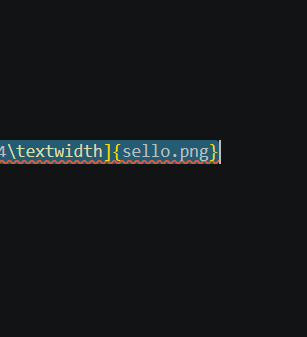
\includegraphics[width=0.4\textwidth]{sello.png}
\end{center}

\vfill

% Fecha abajo
\begin{center}
\today
\end{center}

\newpage

\newpage
\tableofcontents
\newpage

\begin{figure}[htbp]
    \centering
    
\includegraphics[width=0.8\textwidth]{./image.png}
    \caption{Sistema utilizado 6 núcleos.}
    \label{fig:mi_imagen}
\end{figure}







\section{Ejercicios}

\begin{enumerate}
	\item \textbf{Cuestión 1.}

\textbf{a)} Indicar qué pasos habría que llevar a cabo para paralelizar el algoritmo con MPI (no es necesario indicar las primitivas de comunicación). Puedes desarrollar la cuestión de dos maneras: (1) escribir las modificaciones que deberían realizarse sobre cada parte del código secuencial para implementar el modelo de islas, o (2) elaborar un esquema en pseudocódigo que resuma el paralelismo implementado en este modelo. En cualquier caso, tener en cuenta el patrón de computación y comunicaciones entre procesos, desde la lectura inicial de parámetros de entrada, el intercambio de información entre procesos durante el desarrollo del algoritmo, la computación en paralelo, y la comunicación final de resultados.


\medskip
\noindent\textbf{Esquema en pseudocódigo}\par
\smallskip
 
\begin{algorithm}[H]
\caption{Programa principal (\texttt{main})}
\begin{algorithmic}[1]
\State \texttt{MPI\_Init}
\State $rank \gets$ \texttt{MPI\_Comm\_rank}; \quad $size \gets$ \texttt{MPI\_Comm\_size}
\State Todos: leer de los argumentos $n, m, n\_gen, tam\_pob, m\_rate, NGM, NEM$
\If{$rank = 0$}
    \State Leer la matriz de distancias $d$ del fichero
\EndIf
\State Enviar $d$ del proceso 0 al resto de procesos
\State \texttt{MPI\_Barrier}; \quad $t_0 \gets$ \texttt{MPI\_Wtime}
\State $fitness \gets$ \Call{aplicar\_mh}{$d, n, m, n\_gen, tam\_pob, m\_rate, sol, NGM, NEM$}
\State \texttt{MPI\_Barrier}; \quad $t_1 \gets$ \texttt{MPI\_Wtime}
\If{$rank = 0$}
    \State Escribir la solución $sol$, el $fitness$ y el tiempo $t_1 - t_0$
\EndIf
\State \texttt{MPI\_Finalize}
\end{algorithmic}
\end{algorithm}
 
\begin{algorithm}[H]
\caption{Algoritmo evolutivo con modelo de islas (\texttt{aplicar\_mh})}
\begin{algorithmic}[1]
\Function{aplicar\_mh}{$d, n, m, n\_gen, tam\_pob, m\_rate, sol, NGM, NEM$}
    \State Inicializar la semilla aleatoria (distinta en cada proceso)
    \State $tam\_local \gets tam\_pob / size$ \Comment{$+1$ en los primeros $tam\_pob \bmod size$ procesos}
    \State Crear la isla local con $tam\_local$ individuos aleatorios
    \State Calcular el fitness de cada individuo y ordenar la isla
    \State $continuar \gets$ \textbf{cierto}; \quad $g \gets 0$
    \While{$g < n\_gen$ \textbf{y} $continuar$}
        \For{$k \gets 1$ \textbf{hasta} $NGM$} \Comment{sin pasar de $n\_gen$}
            \State Cruzar, mutar, recalcular el fitness y ordenar la isla
            \State $g \gets g + 1$
        \EndFor
        \State \textit{--- Migración ---}
        \State Cada isla envía sus $NEM$ mejores individuos al proceso 0
        \If{$rank = 0$}
            \State Juntar los $NEM \cdot size$ individuos recibidos y ordenarlos
            \State Decidir si se ha alcanzado la convergencia $\rightarrow continuar$
        \EndIf
        \State El proceso 0 envía a todas las islas los $NEM$ mejores y $continuar$
        \State Cada isla sustituye sus $NEM$ peores individuos por los recibidos
        \State Reordenar la isla
    \EndWhile
    \State Cada isla envía su mejor individuo al proceso 0
    \If{$rank = 0$}
        \State Elegir el mejor individuo global y copiarlo en $sol$
    \EndIf
    \State \Return fitness del mejor individuo
\EndFunction
\end{algorithmic}
\end{algorithm}
 
\medskip
\noindent\textbf{Justificación}\par
\smallskip
 
En primer lugar, en el \texttt{main} se hace el \texttt{MPI\_Init} para arrancar MPI y después cada proceso obtiene su número de proceso (\texttt{rank}) y cuántos procesos hay en total (\texttt{size}). Todos los procesos ejecutan el mismo programa, así que el \texttt{rank} es lo que nos permite que cada uno haga una cosa distinta cuando haga falta, por ejemplo, que solo el proceso 0 haga ciertas tareas.
 
Después se leen los parámetros. Cada proceso los lee directamente de los argumentos del programa, porque todos los reciben igual y así no hace falta enviarlos. La matriz de distancias la lee solo el proceso 0 del fichero y luego la envía al resto, ya que todos la necesitan para calcular el fitness. Esto solo se hace una vez al principio, así que apenas afecta al tiempo.
 
Antes de empezar el algoritmo ponemos una barrera y tomamos el tiempo inicial, y al terminar ponemos otra barrera antes de tomar el tiempo final. Así nos aseguramos de que todos empiezan a la vez y de que el tiempo se mide cuando ha terminado el proceso más lento.
 
Ya en \texttt{aplicar\_mh}, cada proceso crea su propia isla, que es su parte de la población. Si la población no se puede repartir de forma exacta, a algunos procesos les toca un individuo más, para que todos tengan más o menos el mismo trabajo. Cada isla genera sus propios individuos en vez de que el proceso 0 lo haga todo y los reparta, porque así también se reparte ese trabajo y nos ahorramos enviar muchos datos. Cada proceso usa una semilla aleatoria distinta para que las islas no sean todas iguales. El proceso 0 también tiene su isla y trabaja como los demás, para no desaprovecharlo.
 
Luego empieza el bucle principal. Cada isla hace por su cuenta lo mismo que hacíamos en la P0 (cruzar, mutar, calcular el fitness y ordenar) durante NGM generaciones, sin comunicarse con nadie. Aquí es donde se gana tiempo, porque cada proceso solo trabaja con una parte de la población.
 
Cada NGM generaciones se hace la migración. Cada isla envía sus NEM mejores individuos al proceso 0, que los junta con los suyos, los ordena y envía los NEM mejores a todas las islas. Cada isla pone esos individuos en el lugar de sus peores y vuelve a ordenar su población, para que los nuevos queden en su sitio y no se pierdan.
 
Además, la decisión de parar el algoritmo la toma el proceso 0 en cada migración, mirando el mejor fitness de todos, y se la comunica al resto. Si cada isla decidiera por su cuenta, una podría parar mientras otra sigue y el programa se quedaría bloqueado esperando mensajes.
 
Por último, cada isla envía su mejor individuo al proceso 0, que se queda con el mejor de todos como solución final. El proceso 0 escribe el resultado y el tiempo, y todos los procesos terminan con \texttt{MPI\_Finalize}.
 
 


\vspace{0.5cm}

\textbf{b)} Las primitivas como \texttt{MPI\_Send} para comunicaciones con paso de mensajes pueden enviar arrays de datos del mismo tipo a condición de que estos estén contiguos en memoria. El código actual implementa la población como un array de punteros a \texttt{Individuo} con lo que los datos pueden estar en posiciones no contiguas de memoria. Como consecuencia se puede producir un error en el envío de poblaciones o subpoblaciones de individuos. Modifica el código como consideres mejor para solucionar este inconveniente, teniendo en cuenta que puedes cambiar de población de \texttt{*Individuo} a \texttt{Individuo} o reservar memoria dinámica auxiliar contigua y apuntar a ella para crear la población.

% --- Respuesta del apartado b) ---

% --- Respuesta del apartado b) ---

\medskip
\noindent\textbf{Problema}\par
\smallskip

MPI solo puede enviar varios datos en un mismo mensaje si están seguidos en memoria. En nuestro código la población era un array de punteros, y cada individuo se creaba con su propio \texttt{malloc}, así que cada uno estaba en un sitio distinto de la memoria. Además, dentro de cada individuo el array de genes también era un puntero a otra zona. Si intentáramos enviar la población así, en realidad estaríamos enviando direcciones de memoria, que en el otro proceso no sirven para nada.

Para solucionarlo, el enunciado da dos opciones: cambiar la población a un array de \texttt{Individuo} en vez de punteros, o reservar un bloque de memoria seguido y hacer que los punteros apunten a él. Nosotros hemos elegido la segunda. A continuación se muestran los cambios realizados.


% cambio 1: struct Individuo

\medskip
\noindent\textbf{Estructura \texttt{Individuo} (\texttt{mh.h})}\par
\smallskip

\noindent\textbf{Antes:}
\begin{lstlisting}[style=EstiloC]
typedef struct {
    int *array_int;
    double fitness;
} Individuo;
\end{lstlisting}

\noindent\textbf{Después:}
\begin{lstlisting}[style=EstiloC]
#define MAX_M 1000   // tamano maximo de un individuo (>= el mayor m usado)

typedef struct {
    int array_int[MAX_M];   // los genes van dentro del struct
    double fitness;
} Individuo;
\end{lstlisting}

\textbf{Justificación:} El campo \texttt{array\_int} ha pasado de ser un puntero a ser un array de tamaño fijo, con un tamaño máximo \texttt{MAX\_M} suficiente para los problemas que vamos a usar. Así los genes están dentro del propio individuo y cada individuo es un único bloque de memoria que se puede enviar de una vez. Esto además es necesario para poder usar el tipo de datos de \texttt{derivados\_mpi.c}. Hay que tener cuidado de no poner un \texttt{MAX\_M} mucho más grande de lo necesario, porque cada individuo ocuparía más memoria y se enviarían más datos de los que hacen falta.

\vspace{0.5cm}

% cambio 2: crear_individuo

\medskip
\noindent\textbf{Función \texttt{crear\_individuo}}\par
\smallskip

\noindent\textbf{Antes:}
\begin{lstlisting}[style=EstiloC]
int *crear_individuo(int n, int m)
{
    int i=0, value;
    int *individuo = (int *) malloc(m * sizeof(int));

    // inicializa array de elementos
    memset(individuo, -1, m * sizeof(int));

    while(i < m) {
        value = aleatorio(n);
        // si el nuevo elemento no esta en el array...
        if(!find_element(individuo, i, value)) {
            individuo[i] = value;  // lo incluimos
            i++;
        }
    }
    return individuo;
}
\end{lstlisting}

\noindent\textbf{Después:}
\begin{lstlisting}[style=EstiloC]
void crear_individuo(int n, int m, int *individuo)
{
    int i=0, value;

    // inicializa array de elementos (ya reservado dentro del struct)
    memset(individuo, -1, m * sizeof(int));

    while(i < m) {
        value = aleatorio(n);
        // si el nuevo elemento no esta en el array...
        if(!find_element(individuo, i, value)) {
            individuo[i] = value;  // lo incluimos
            i++;
        }
    }
}
\end{lstlisting}

\textbf{Justificación:} Antes la función reservaba memoria para los genes y devolvía el puntero. Ahora los genes ya están dentro del individuo, así que la función solo se encarga de rellenarlos con valores aleatorios sin repetir. Por eso desaparecen el \texttt{malloc} y el \texttt{return}, y la función recibe como parámetro el array que tiene que rellenar.

\vspace{0.5cm}


% cambio 3: creación de la población

\medskip
\noindent\textbf{Creación de la población en \texttt{aplicar\_mh}}\par
\smallskip

\noindent\textbf{Antes:}
\begin{lstlisting}[style=EstiloC]
// crea poblacion inicial (array de individuos)
Individuo **poblacion = (Individuo **) malloc(tam_pob * sizeof(Individuo *));
assert(poblacion);

// crea cada individuo (array de enteros aleatorios)
for(i = 0; i < tam_pob; i++) {
    poblacion[i] = (Individuo *) malloc(sizeof(Individuo));
    poblacion[i]->array_int = crear_individuo(n, m);

    // calcula el fitness del individuo
    fitness(d, poblacion[i], n, m);
}
\end{lstlisting}

\noindent\textbf{Después:}
\begin{lstlisting}[style=EstiloC]
assert(m <= MAX_M);   // el individuo tiene que caber en el array estatico

// bloque contiguo con todos los individuos (necesario para MPI)
Individuo *bloque = (Individuo *) malloc(tam_pob * sizeof(Individuo));
assert(bloque);

// array de punteros al bloque: es lo que se ordena con qsort
Individuo **poblacion = (Individuo **) malloc(tam_pob * sizeof(Individuo *));
assert(poblacion);

// crea cada individuo (array de enteros aleatorios)
for(i = 0; i < tam_pob; i++) {
    poblacion[i] = &bloque[i];
    crear_individuo(n, m, poblacion[i]->array_int);

    // calcula el fitness del individuo
    fitness(d, poblacion[i], n, m);
}
\end{lstlisting}

\textbf{Justificación:} Reservamos con un solo \texttt{malloc} un bloque con espacio para todos los individuos, de forma que quedan uno detrás de otro, y seguimos teniendo el array de punteros, donde cada puntero apunta a un individuo del bloque. También se ha añadido un \texttt{assert} para que el programa se pare con un mensaje claro si se ejecuta con un $m$ mayor que \texttt{MAX\_M}.

La razón principal de elegir esta opción en vez de cambiar la población a un array de \texttt{Individuo} es la ordenación. En cada generación se ordena la población con \texttt{qsort}, y con punteros lo que se mueve son los punteros, que ocupan muy poco. Si la población fuera un array de individuos, el \texttt{qsort} tendría que mover individuos enteros, que con el array de genes dentro ocupan bastante más, y eso se haría en todas las generaciones. Además, con esta opción el resto del código (\texttt{cruzar}, \texttt{mutar}, \texttt{fitness} y el bucle principal) se queda igual, así que es más difícil meter errores.

\vspace{0.5cm}


% cambio 4: liberación de memoria

\medskip
\noindent\textbf{Liberación de memoria en \texttt{aplicar\_mh}}\par
\smallskip

\noindent\textbf{Antes:}
\begin{lstlisting}[style=EstiloC]
// se libera la memoria reservada
for (int i=0; i<tam_pob ; i++){
    free(poblacion[i]->array_int);
    free(poblacion[i]);
}
free(poblacion);
\end{lstlisting}

\noindent\textbf{Después:}
\begin{lstlisting}[style=EstiloC]
// se libera la memoria reservada (un solo bloque y el array de punteros)
free(bloque);
free(poblacion);
\end{lstlisting}

\textbf{Justificación:} Antes había un bucle que liberaba los genes de cada individuo y cada individuo por separado. Ahora solo hay dos reservas, la del bloque y la del array de punteros, así que basta con dos \texttt{free}. Si dejáramos el bucle antiguo, el programa fallaría al intentar liberar memoria que no se reservó por separado.

\vspace{0.5cm}

% cambio 5: funciones nuevas

\medskip
\noindent\textbf{Funciones nuevas \texttt{copiar\_mejores} y \texttt{reemplazar\_peores}}\par
\smallskip


\begin{lstlisting}[style=EstiloC]
// Copia los k mejores individuos (poblacion ya ordenada) a un buffer contiguo
void copiar_mejores(Individuo **poblacion, Individuo *buffer, int k)
{
    for (int i = 0; i < k; i++)
        buffer[i] = *poblacion[i];
}

// Sustituye los k peores individuos por los recibidos y reordena la poblacion
void reemplazar_peores(Individuo **poblacion, int tam, Individuo *recibidos, int k)
{
    for (int i = 0; i < k; i++)
        *poblacion[tam - 1 - i] = recibidos[i];
    qsort(poblacion, tam, sizeof(Individuo *), comp_fitness);
}
\end{lstlisting}

\textbf{Justificación:} La opción que elegimos tiene un pequeño inconveniente. Al ordenar, se reordenan los punteros pero los individuos no se mueven dentro del bloque, así que después de ordenar los mejores ya no están seguidos en memoria. Para solucionarlo hemos creado la función \texttt{copiar\_mejores}, que antes de cada envío copia los NEM mejores individuos a un buffer auxiliar, donde sí quedan seguidos y se pueden enviar en un solo mensaje. Esta copia solo se hace en las migraciones y solo para unos pocos individuos, así que cuesta mucho menos que mover individuos enteros en cada ordenación.

La función \texttt{reemplazar\_peores} se usará al recibir los individuos de la migración. Copia los individuos recibidos encima de los peores de la isla y después vuelve a ordenar. Es importante que se copie el contenido y no que se cambie el puntero para que apunte al buffer recibido, porque ese buffer se vuelve a usar en la siguiente migración y los individuos cambiarían solos. Además, así todos los individuos siguen estando dentro del bloque de la isla.

\vspace{0.5cm}

% cambio 6: comp_fitness

\medskip
\noindent\textbf{Función \texttt{comp\_fitness}}\par
\smallskip

\noindent\textbf{Antes:}
\begin{lstlisting}[style=EstiloC]
int comp_fitness(const void *a, const void *b) {
    /* qsort pasa un puntero al elemento que esta ordenando */
    return (*(Individuo **)b)->fitness - (*(Individuo **)a)->fitness;
}
\end{lstlisting}

\noindent\textbf{Después:}
\begin{lstlisting}[style=EstiloC]
int comp_fitness(const void *a, const void *b) {
    /* qsort pasa un puntero al elemento que esta ordenando */
    double fa = (*(Individuo **)a)->fitness;
    double fb = (*(Individuo **)b)->fitness;
    return (fb > fa) - (fb < fa);   // orden descendente sin truncar a int
}
\end{lstlisting}

\textbf{Justificación:} Aprovechando estos cambios hemos corregido esta función, que es la que usa el \texttt{qsort} para ordenar. Antes restaba los dos fitness, que son \texttt{double}, y devolvía el resultado como \texttt{int}. Esto hacía que las diferencias pequeñas se quedaran en 0 y que con valores grandes el resultado pudiera salir mal, por lo que la población podía quedar mal ordenada. Ahora compara los dos valores directamente y devuelve -1, 0 o 1. Esto es más importante con MPI, porque si el proceso 0 ordena mal la mezcla podría enviar a todas las islas individuos que no son los mejores.

\vspace{0.5cm}



\newpage
\item \textbf{Cuestión 2.} Paralelizar el algoritmo evolutivo utilizando primitivas de comunicación síncrona. Hacer uso de las constantes \texttt{MPI\_ANY\_SOURCE} o \texttt{MPI\_STATUS\_IGNORE}, si se considera conveniente, para evitar que el proceso 0 quede ocioso durante la recepción de mensajes del resto de procesos. Analizar las prestaciones que se obtienen al variar el número de procesos. Tener en cuenta el punto (3) en Observaciones para determinar los valores de NEM y NGM.

% --- Respuesta de la cuestión 2 ---


Se ha implementado el modelo de islas de la cuestión 1a usando comunicaciones punto a punto síncronas: todos los envíos se hacen con \texttt{MPI\_Ssend} (envío síncrono, que termina cuando el receptor ha empezado a recibir) y las recepciones con \texttt{MPI\_Recv}. Los individuos se envían con el tipo derivado de \texttt{derivados\_mpi.c}, cuya función \texttt{crear\_tipo\_datos} se ha copiado en \texttt{mh.c}. Para compilar y ejecutar se han adaptado el \texttt{Makefile} (con \texttt{mpicc} y \texttt{mpirun}) y el \texttt{run.sh}. A continuación se muestran las partes del código modificadas.

% cambio 1: inicialización de MPI

\medskip
\noindent\textbf{Inicialización de MPI y parámetros (\texttt{main.c})}\par
\smallskip

\begin{lstlisting}[style=EstiloC]
MPI_Init(&argc, &argv);
MPI_Comm_rank(MPI_COMM_WORLD, &rank);
MPI_Comm_size(MPI_COMM_WORLD, &size);
...
int NGM = atoi(argv[6]);   // cada cuántas generaciones hay migración
int NEM = atoi(argv[7]);   // cuántos individuos migran de cada isla
...
assert(tam_pob / size >= 4);
assert(NEM <= tam_pob / size);
\end{lstlisting}

\textbf{Justificación:} Se arranca MPI y cada proceso obtiene su identificador y el número de procesos, que es lo que permite que cada uno haga una parte distinta. NGM y NEM se pasan como argumentos para poder probar distintos valores sin recompilar, y todos los procesos los leen de la línea de comandos, así que no hace falta enviarlos. Los \texttt{assert} comprueban que cada isla tenga al menos 4 individuos para poder cruzar y que NEM quepa en la isla más pequeña.

\vspace{0.5cm}

% cambio 2: matriz de distancias

\medskip
\noindent\textbf{Envío de la matriz de distancias (\texttt{main.c})}\par
\smallskip

\begin{lstlisting}[style=EstiloC]
int tam_d = (n*n - n)/2;
double *d;
if(rank == 0) {
	d = read_distances(n);
	for(int dest = 1; dest < size; dest++) {
		MPI_Ssend(d, tam_d, MPI_DOUBLE, dest, 0, MPI_COMM_WORLD);
	}
} else {
	d = (double *) malloc(tam_d * sizeof(double));
	assert(d);
	MPI_Recv(d, tam_d, MPI_DOUBLE, 0, 0, MPI_COMM_WORLD, MPI_STATUS_IGNORE);
}
\end{lstlisting}

\textbf{Justificación:} Con \texttt{mpirun} la entrada estándar solo le llega al proceso 0, así que solo él lee la matriz y la envía al resto, que la necesitan para calcular el fitness. Se envía entera en un solo mensaje porque es un array contiguo. Solo se hace una vez y queda fuera de la medida de tiempo.

\vspace{0.5cm}

% cambio 3: tiempos

\medskip
\noindent\textbf{Toma de tiempos (\texttt{main.c})}\par
\smallskip

\begin{lstlisting}[style=EstiloC]
MPI_Barrier(MPI_COMM_WORLD);
#ifdef TIME
	double ti = mseconds();
#endif

double value = aplicar_mh(d, n, m, n_gen, tam_pob, m_rate, sol, NGM, NEM);

MPI_Barrier(MPI_COMM_WORLD);
#ifdef TIME
	double tf = mseconds();
#endif
\end{lstlisting}

\textbf{Justificación:} Como indica la observación 1, se pone una barrera antes de cada toma de tiempo: la primera para que todos empiecen a la vez y la segunda para medir cuando ha terminado el proceso más lento. Después solo el proceso 0 escribe el tiempo y la solución, y todos terminan con \texttt{MPI\_Finalize}.

\vspace{0.5cm}

% cambio 4: islas

\medskip
\noindent\textbf{Creación de las islas (\texttt{aplicar\_mh})}\par
\smallskip

\begin{lstlisting}[style=EstiloC]
srand(time(NULL) + getpid() + rank * 1000);
...
int tam_local = tam_pob / size;
if (rank < tam_pob % size)
	tam_local++;

Individuo *bloque = (Individuo *) malloc(tam_local * sizeof(Individuo));
...
for(i = 0; i < tam_local; i++) {
	poblacion[i] = &bloque[i];
	crear_individuo(n, m, poblacion[i]->array_int);
	...
}
\end{lstlisting}

\textbf{Justificación:} Cada proceso crea su propia isla con \texttt{tam\_pob/size} individuos, y si no es divisible los primeros procesos tienen uno más, para que la carga quede equilibrada. Cada isla se genera en su proceso en vez de repartirla el 0, así esa parte también se hace en paralelo y no hay que enviar la población inicial. Se suma el \texttt{rank} a la semilla para que todas las islas sean distintas.

\vspace{0.5cm}

% cambio 5: bucle principal

\medskip
\noindent\textbf{Bucle de evolución (\texttt{aplicar\_mh})}\par
\smallskip

\begin{lstlisting}[style=EstiloC]
while (g < n_gen && continuar)
{
	int gen_bloque = 0;
	for (k = 0; k < NGM && g < n_gen; k++, g++, gen_bloque++)
	{
		...
	}

	// Migración
	...
}
\end{lstlisting}

\textbf{Justificación:} El bucle de la P0 se divide en bloques de NGM generaciones. Dentro de cada bloque cada isla cruza, muta, calcula el fitness y ordena igual que en la P0, pero solo con sus \texttt{tam\_local} individuos y sin comunicarse, que es donde se gana tiempo. Al final de cada bloque se hace la migración. Todos los procesos hacen las mismas generaciones, así que llegan a la migración a la vez sin tener que comunicar \texttt{g}.

\vspace{0.5cm}

% cambio 6: migración

\medskip
\noindent\textbf{Migración (\texttt{aplicar\_mh})}\par
\smallskip

\begin{lstlisting}[style=EstiloC]
copiar_mejores(poblacion, emigrantes, NEM);

if (rank == 0) {
	for (i = 0; i < NEM; i++)
		mezcla[i] = emigrantes[i];

	for (k = 1; k < size; k++) {
		MPI_Recv(&mezcla[k * NEM], NEM, individuo_type, MPI_ANY_SOURCE, 1,
				 MPI_COMM_WORLD, MPI_STATUS_IGNORE);
	}

	for (i = 0; i < NEM * size; i++)
		p_mezcla[i] = &mezcla[i];
	qsort(p_mezcla, NEM * size, sizeof(Individuo *), comp_fitness);
	copiar_mejores(p_mezcla, inmigrantes, NEM);

	double fitness_esperado = fitness_modelo * (1 + PCT_CONVER);
	if (p_mezcla[0]->fitness > fitness_esperado) {
		fitness_modelo = p_mezcla[0]->fitness;
		ngeneracion = 0;
	} else {
		ngeneracion += gen_bloque;
	}
	continuar = (ngeneracion < NGENERACIONES_ATRAS);
	...
	for (k = 1; k < size; k++) {
		MPI_Ssend(inmigrantes, NEM, individuo_type, k, 2, MPI_COMM_WORLD);
		MPI_Ssend(&continuar, 1, MPI_INT, k, 3, MPI_COMM_WORLD);
	}
} else {
	MPI_Ssend(emigrantes, NEM, individuo_type, 0, 1, MPI_COMM_WORLD);
	MPI_Recv(inmigrantes, NEM, individuo_type, 0, 2, MPI_COMM_WORLD, MPI_STATUS_IGNORE);
	MPI_Recv(&continuar, 1, MPI_INT, 0, 3, MPI_COMM_WORLD, MPI_STATUS_IGNORE);
}

reemplazar_peores(poblacion, tam_local, inmigrantes, NEM);
\end{lstlisting}

\textbf{Justificación:} Cada isla copia sus NEM mejores a un buffer contiguo con \texttt{copiar\_mejores} y los envía al proceso 0 en un solo mensaje. El proceso 0 añade los suyos directamente (no se envía mensajes a sí mismo), ordena la mezcla y devuelve a todas las islas los NEM mejores globales, que sustituyen a sus peores individuos con \texttt{reemplazar\_peores}.

El proceso 0 recibe con \texttt{MPI\_ANY\_SOURCE}, es decir, en el orden en que llegan los mensajes, y guarda cada uno en el siguiente hueco libre de la mezcla. Así no se queda parado esperando a una isla lenta mientras otras ya han enviado, que es lo que pide el enunciado. Como no importa de qué isla viene cada mensaje, no se necesita el \texttt{status} y se usa \texttt{MPI\_STATUS\_IGNORE}.

La convergencia la decide solo el proceso 0, con el mejor fitness global, y la envía al resto en \texttt{continuar}. Si cada isla decidiera por su cuenta, una podría parar mientras las demás le envían mensajes y el programa se bloquearía. Como solo se comprueba en las migraciones, si no hay mejora se suman las generaciones de todo el bloque. Tampoco hay interbloqueo con los envíos síncronos, porque las islas siempre envían antes de recibir y el proceso 0 siempre recibe antes de enviar.

\vspace{0.5cm}

% cambio 7: resultado final

\medskip
\noindent\textbf{Resultado final (\texttt{aplicar\_mh})}\par
\smallskip

\begin{lstlisting}[style=EstiloC]
Individuo mejor = *poblacion[0];
if (rank == 0) {
	Individuo recibido;
	for (k = 1; k < size; k++) {
		MPI_Recv(&recibido, 1, individuo_type, MPI_ANY_SOURCE, 4, MPI_COMM_WORLD, MPI_STATUS_IGNORE);
		if (recibido.fitness > mejor.fitness)
			mejor = recibido;
	}
} else {
	MPI_Ssend(&mejor, 1, individuo_type, 0, 4, MPI_COMM_WORLD);
}
\end{lstlisting}

\textbf{Justificación:} Al terminar, cada isla envía su mejor individuo al proceso 0, que se queda con el de mayor fitness como solución. También se usa \texttt{MPI\_ANY\_SOURCE}, porque el orden no importa: solo hay que quedarse con el máximo.

\vspace{0.5cm}

\medskip
\noindent\textbf{Elección de NGM y NEM}\par
\smallskip

% >>> DATO: tabla de NGM/NEM. Media de las 3 repeticiones de cada combinación (tiempo y Distance)
Se han probado NGM $\in \{5, 10, 20, 50\}$ y NEM $\in \{1, 3, 5\}$ con 6 procesos y la instancia \texttt{1000 400 200 100 0.3}, repitiendo cada combinación 3 veces (Tabla~\ref{tab:ngm_nem}).

\begin{table}[htbp]
\centering
\begin{tabular}{c|ccc|ccc}
\toprule
& \multicolumn{3}{c|}{\textbf{Tiempo medio (s)}} & \multicolumn{3}{c}{\textbf{Fitness medio}} \\
\textbf{NGM} & NEM=1 & NEM=3 & NEM=5 & NEM=1 & NEM=3 & NEM=5 \\
\midrule
5  & 0.150 & 0.147 & 0.143 & 4\,017\,865 & 4\,017\,682 & 4\,017\,575 \\
10 & 0.193 & 0.193 & 0.197 & 4\,015\,756 & 4\,016\,673 & 4\,018\,129 \\
20 & 0.190 & 0.193 & 0.187 & 4\,015\,302 & 4\,015\,518 & 4\,016\,630 \\
50 & 0.457 & 0.443 & 0.450 & 4\,020\,613 & 4\,018\,482 & 4\,020\,628 \\
\bottomrule
\end{tabular}
\caption{Pruebas de NGM y NEM con 6 procesos ($n=1000$, $m=400$, $n\_gen=200$, $tam\_pob=100$, $m\_rate=0.3$). Media de 3 ejecuciones.}
\label{tab:ngm_nem}
\end{table}

% >>> DATO: revisar las cifras de este párrafo y los valores elegidos
El fitness es prácticamente igual en todas las combinaciones (diferencias de alrededor del 0{,}1\,\%, del mismo orden que la variación entre repeticiones) y NEM no influye ni en el tiempo ni en el fitness. El tiempo crece con NGM, pero no por las comunicaciones: como la convergencia solo se comprueba en las migraciones, el algoritmo no puede parar antes de acumular 15 generaciones sin mejora en bloques de NGM (mínimo de 15, 20, 20 y 50 generaciones), y los tiempos son casi proporcionales a esos valores. Es decir, el coste por generación es el mismo y las comunicaciones apenas cuestan. Elegimos \textbf{NGM = 10 y NEM = 3}: NGM = 50 más que duplica el tiempo sin mejorar el fitness de forma apreciable, y entre 5, 10 y 20 tomamos el valor intermedio, que deja evolucionar las islas de forma independiente pero intercambia individuos con frecuencia. NEM = 3 es un valor intermedio que reparte los mejores sin sustituir gran parte de cada isla.

\vspace{0.5cm}

\medskip
\noindent\textbf{Resultados}\par
\smallskip

% >>> DATO: máquina, instancia, procesos y repeticiones
Los experimentos se han realizado en un Intel Core i7-1355U (10 núcleos físicos: 2 de rendimiento y 8 de eficiencia, 12~MiB de caché L3) con la instancia \texttt{2000 800 400 200 0.3}, NGM = 10 y NEM = 3, mediante los scripts \texttt{prestaciones.sh} y \texttt{prestaciones\_fijo.sh}. Se dan dos versiones: la normal, con el criterio de convergencia, y una de trabajo fijo que siempre hace 60 generaciones. Esta segunda se obtiene compilando con \texttt{make mpi\_fijo}, que define \texttt{SIN\_CONVERGENCIA} y hace que en \texttt{mh.c} se use un \texttt{NGENERACIONES\_ATRAS} muy grande, de forma que nunca converge. Es necesaria porque con convergencia el número de generaciones cambia de una ejecución a otra, y así no siempre se compara el mismo trabajo. El tiempo de referencia del speed-up es el del algoritmo paralelo con 1 proceso.

% >>> DATO: copiar de output/prestaciones.txt y output/prestaciones_fijo.txt
\begin{table}[htbp]
\centering
\begin{tabular}{c|ccc|ccc}
\toprule
& \multicolumn{3}{c|}{\textbf{Con convergencia}} & \multicolumn{3}{c}{\textbf{Trabajo fijo (60 gen.)}} \\
\textbf{n\_procesos} & t\_ejec (s) & speed-up & eficiencia & t\_ejec (s) & speed-up & eficiencia \\
\midrule
1 & 5.364 & 1.00 & 1.00 & 13.300 & 1.00 & 1.00 \\
2 & 4.048 & 1.33 & 0.66 & 10.580 & 1.26 & 0.63 \\
4 & 3.758 & 1.43 & 0.36 & 10.363 & 1.28 & 0.32 \\
6 & 3.382 & 1.59 & 0.26 & 9.820 & 1.35 & 0.23 \\
8 & 3.466 & 1.55 & 0.19 & 9.407 & 1.41 & 0.18 \\
\bottomrule
\end{tabular}
\caption{Prestaciones con $n=2000$, $m=800$, $tam\_pob=200$, $m\_rate=0.3$, NGM = 10 y NEM = 3. Media de 5 ejecuciones (convergencia) y 3 (trabajo fijo).}
\label{tab:c2_prestaciones}
\end{table}

% >>> DATO: cambiar las coordinates (np,valor) con los speed-up de la tabla
\begin{figure}[htbp]
\centering
\begin{tikzpicture}
\begin{axis}[
    width=0.6\textwidth, height=6cm,
    xlabel={Número de procesos}, ylabel={Speed-up},
    xtick={1,2,4,6,8}, ymin=0, ymax=4, grid=major,
    legend pos=north west, legend style={font=\scriptsize}]
\addplot[mark=*, color=primary, thick] coordinates {(1,1.00) (2,1.33) (4,1.43) (6,1.59) (8,1.55)};
\addplot[mark=square*, color=secondary, thick] coordinates {(1,1.00) (2,1.26) (4,1.28) (6,1.35) (8,1.41)};
\addplot[dashed, color=gray] coordinates {(1,1) (8,8)};
\legend{Con convergencia, Trabajo fijo, Ideal}
\end{axis}
\end{tikzpicture}
\caption{Speed-up al variar el número de procesos.}
\label{fig:c2_speedup}
\end{figure}

\vspace{0.5cm}

\medskip
\noindent\textbf{Análisis}\par
\smallskip

% >>> DATO: revisar las cifras de este apartado con las nuevas tablas
El tiempo baja al aumentar los procesos, pero mucho menos de lo ideal: el speed-up máximo es de 1.59 (convergencia) y 1.41 (trabajo fijo), y la eficiencia cae por debajo de 0.25 a partir de 6 procesos. A partir de 4 procesos la mejora es mínima.

La causa no son las comunicaciones, ya que solo se envían 3 individuos por isla en cada migración y las pruebas de NGM muestran que el coste por generación no cambia con la frecuencia de migración. Las causas más probables son de la máquina:

\begin{itemize}
    \item \textbf{Memoria:} cada proceso tiene su copia de la matriz de distancias (unos 16~MB con $n=2000$), que no cabe en la caché L3 de 12~MiB, y los procesos compiten por la caché y el ancho de banda de memoria.
    \item \textbf{Núcleos heterogéneos:} solo hay 2 núcleos de rendimiento. Como en cada migración todos esperan al proceso más lento, los procesos en núcleos de eficiencia frenan al resto.
    \item \textbf{Límite de potencia del portátil:} con más núcleos activos baja la frecuencia de cada uno.
\end{itemize}

% >>> DATO: revisar la recomendación final
Por tanto, en esta máquina los valores más razonables son 2 o 4 procesos.
\newpage
\item \textbf{Cuestión 3.} Modificar la cuestión anterior para que el envío y la recepción de datos se realice mediante el uso de las funciones \texttt{MPI\_Pack} y \texttt{MPI\_Unpack} para empaquetamiento de datos (o cualquier otro método de envío diferente al uso del tipo derivado \texttt{Individuo}, de forma que se envíe en un mismo mensaje toda la estructura de individuo, no varios mensajes con cada parte). Presentar también resultados de los experimentos realizados.

% --- Respuesta de la cuestión 3 ---


\newpage
\item \textbf{Cuestión 4.} Paralelizar el algoritmo evolutivo utilizando primitivas de comunicación asíncrona. Analizar las prestaciones obtenidas al variar el número de procesos.

% --- Respuesta de la cuestión 4 ---


\newpage
\item \textbf{Cuestión 5.} Paralelizar el algoritmo evolutivo utilizando primitivas de comunicación colectiva. Analizar las prestaciones obtenidas al variar el número de procesos.

% --- Respuesta de la cuestión 5 ---


\newpage
\item \textbf{Cuestión 6.} Elegir la mejor configuración de parámetros y tipo de comunicaciones para paralelizar la totalidad del algoritmo. Justificar las decisiones tomadas. De este modo, se pretende tener un código paralelo óptimo en memoria distribuida que se podrá usar para comparar con el código secuencial, y paralelo en memoria compartida e híbrido.

% --- Respuesta de la cuestión 6 ---


\newpage
\item \textbf{Cuestión 7.} Realizar el informe final incluyendo las conclusiones generales y valoración personal sobre el trabajo realizado.

% --- Respuesta de la cuestión 7 ---


\end{enumerate}

\end{document}